% Options for packages loaded elsewhere
\PassOptionsToPackage{unicode}{hyperref}
\PassOptionsToPackage{hyphens}{url}
%
\documentclass[
]{book}
\usepackage{lmodern}
\usepackage{amssymb,amsmath}
\usepackage{ifxetex,ifluatex}
\ifnum 0\ifxetex 1\fi\ifluatex 1\fi=0 % if pdftex
  \usepackage[T1]{fontenc}
  \usepackage[utf8]{inputenc}
  \usepackage{textcomp} % provide euro and other symbols
\else % if luatex or xetex
  \usepackage{unicode-math}
  \defaultfontfeatures{Scale=MatchLowercase}
  \defaultfontfeatures[\rmfamily]{Ligatures=TeX,Scale=1}
\fi
% Use upquote if available, for straight quotes in verbatim environments
\IfFileExists{upquote.sty}{\usepackage{upquote}}{}
\IfFileExists{microtype.sty}{% use microtype if available
  \usepackage[]{microtype}
  \UseMicrotypeSet[protrusion]{basicmath} % disable protrusion for tt fonts
}{}
\makeatletter
\@ifundefined{KOMAClassName}{% if non-KOMA class
  \IfFileExists{parskip.sty}{%
    \usepackage{parskip}
  }{% else
    \setlength{\parindent}{0pt}
    \setlength{\parskip}{6pt plus 2pt minus 1pt}}
}{% if KOMA class
  \KOMAoptions{parskip=half}}
\makeatother
\usepackage{xcolor}
\IfFileExists{xurl.sty}{\usepackage{xurl}}{} % add URL line breaks if available
\IfFileExists{bookmark.sty}{\usepackage{bookmark}}{\usepackage{hyperref}}
\hypersetup{
  pdftitle={Topology Inference for Radial Distribution Feeder based on Power Flow},
  pdfauthor={Jie Xu (s181238)},
  hidelinks,
  pdfcreator={LaTeX via pandoc}}
\urlstyle{same} % disable monospaced font for URLs
\usepackage{longtable,booktabs}
% Correct order of tables after \paragraph or \subparagraph
\usepackage{etoolbox}
\makeatletter
\patchcmd\longtable{\par}{\if@noskipsec\mbox{}\fi\par}{}{}
\makeatother
% Allow footnotes in longtable head/foot
\IfFileExists{footnotehyper.sty}{\usepackage{footnotehyper}}{\usepackage{footnote}}
\makesavenoteenv{longtable}
\usepackage{graphicx}
\makeatletter
\def\maxwidth{\ifdim\Gin@nat@width>\linewidth\linewidth\else\Gin@nat@width\fi}
\def\maxheight{\ifdim\Gin@nat@height>\textheight\textheight\else\Gin@nat@height\fi}
\makeatother
% Scale images if necessary, so that they will not overflow the page
% margins by default, and it is still possible to overwrite the defaults
% using explicit options in \includegraphics[width, height, ...]{}
\setkeys{Gin}{width=\maxwidth,height=\maxheight,keepaspectratio}
% Set default figure placement to htbp
\makeatletter
\def\fps@figure{htbp}
\makeatother
\usepackage[normalem]{ulem}
% Avoid problems with \sout in headers with hyperref
\pdfstringdefDisableCommands{\renewcommand{\sout}{}}
\setlength{\emergencystretch}{3em} % prevent overfull lines
\providecommand{\tightlist}{%
  \setlength{\itemsep}{0pt}\setlength{\parskip}{0pt}}
\setcounter{secnumdepth}{5}
\usepackage{booktabs}
\usepackage{amsthm}
\makeatletter
\def\thm@space@setup{%
  \thm@preskip=8pt plus 2pt minus 4pt
  \thm@postskip=\thm@preskip
}
\makeatother
\usepackage{booktabs}
\usepackage{longtable}
\usepackage{array}
\usepackage{multirow}
\usepackage{wrapfig}
\usepackage{float}
\usepackage{colortbl}
\usepackage{pdflscape}
\usepackage{tabu}
\usepackage{threeparttable}
\usepackage{threeparttablex}
\usepackage[normalem]{ulem}
\usepackage{makecell}
\usepackage{xcolor}
\usepackage[]{natbib}
\bibliographystyle{apalike}

\title{Topology Inference for Radial Distribution Feeder based on Power Flow}
\author{Jie Xu (s181238)}
\date{2020-12-15}

\begin{document}
\maketitle

{
\setcounter{tocdepth}{1}
\tableofcontents
}
\hypertarget{introduction}{%
\chapter{Introduction}\label{introduction}}

\hypertarget{problem-setting}{%
\subsection*{Problem Setting}\label{problem-setting}}
\addcontentsline{toc}{subsection}{Problem Setting}

Available information for topology inference:

\begin{itemize}
\tightlist
\item
  geographical information about buses
\item
  voltage magnitudes of all the phases of all the buses
\item
  some real power injection profiles
\end{itemize}

Association network inference: correlation between buses

\begin{itemize}
\tightlist
\item
  Spurious correlation resulted from correlated profiles.
\item
  Missing measurement.
\end{itemize}

\hypertarget{flowchart}{%
\subsection*{Flowchart}\label{flowchart}}
\addcontentsline{toc}{subsection}{Flowchart}

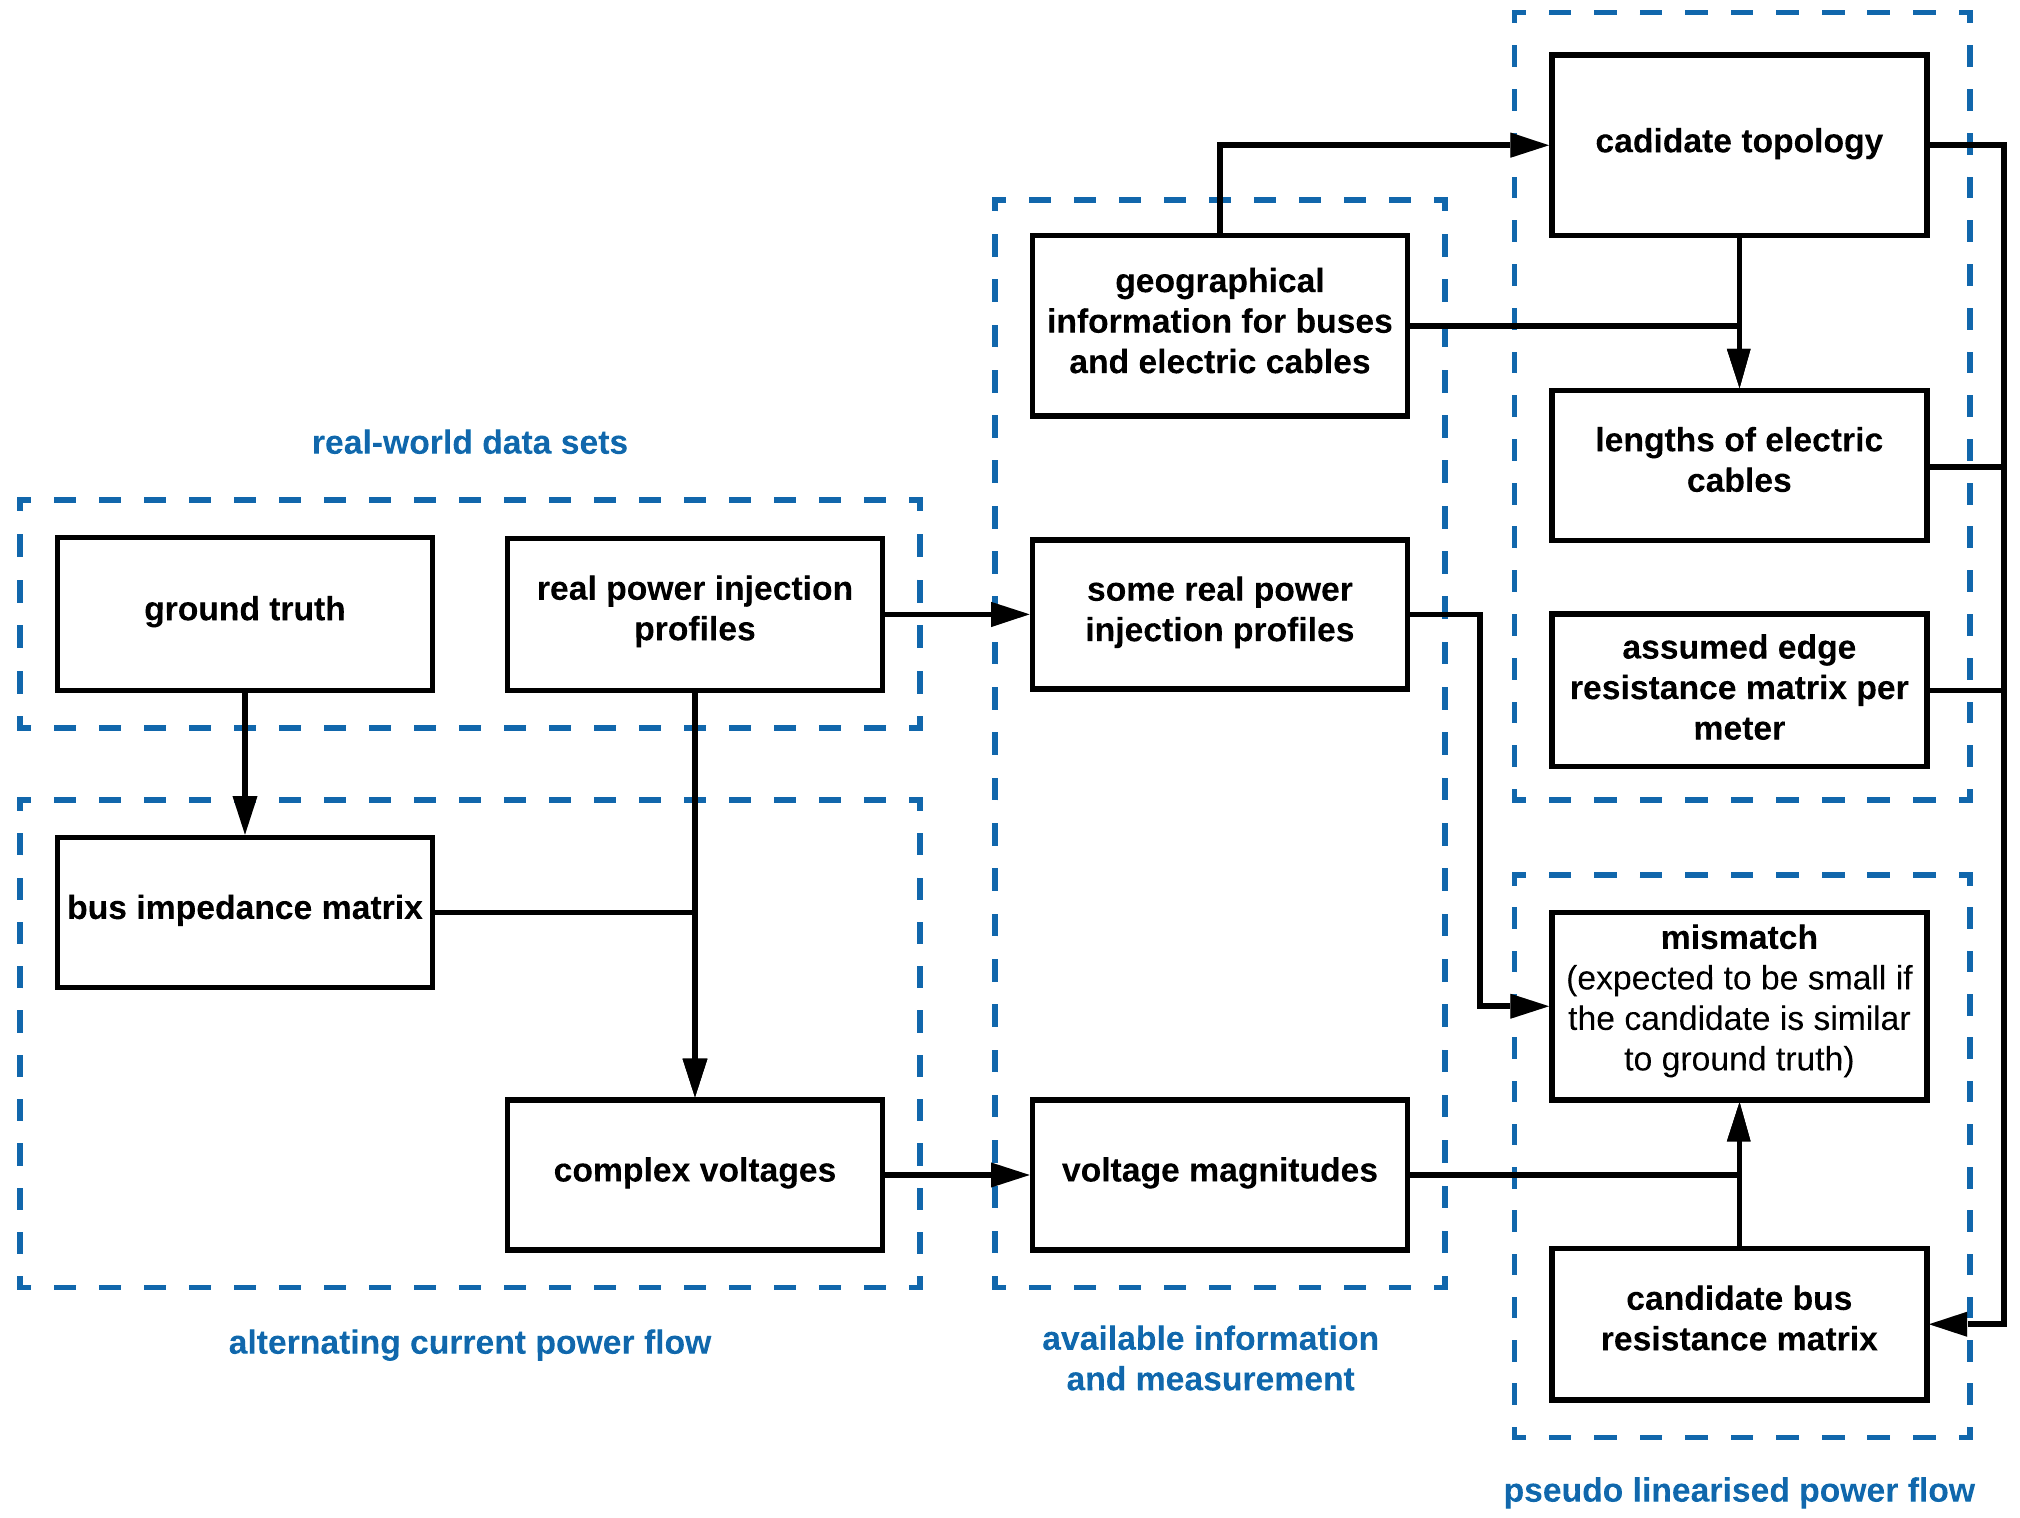
\includegraphics{Pictures/figFlowchart3.png}

\textbf{Ground truth} is to be found in topolgoy inference, but used to simulate
available measurement first.

Two batches of computer programs:

\begin{itemize}
\tightlist
\item
  power flow
\item
  three algorithms to handle directed graphs
\end{itemize}

\hypertarget{radial-distribution-feeder}{%
\chapter{Radial Distribution Feeder}\label{radial-distribution-feeder}}

\begin{itemize}
\tightlist
\item
  bus and edge, \protect\hyperlink{bus-edge}{-\textgreater{} 2.1}
\item
  two special concepts for power flow, \protect\hyperlink{concepts}{-\textgreater{} 2.2}
\item
  case with 70 buses, \protect\hyperlink{case}{-\textgreater{} 2.3}
\end{itemize}

\hypertarget{bus-edge}{%
\section{Bus and Edge}\label{bus-edge}}

\begin{table}[H]
\centering
\begin{tabular}[t]{l|l|l}
\hline
type & definition & examples\\
\hline
edge & transport power from one place to another & cable, transformer, capacitor\\
\hline
conversion element & convert power from or to another form & solar panel, battery\\
\hline
bus & where two edges joint or end of an edge & slack bus, PQ bus, PV bus\\
\hline
\end{tabular}
\end{table}

\begin{itemize}
\tightlist
\item
  Cable.
\item
  One slack bus -\textgreater{} \textbf{root}.
\item
  Ignore conversion elements. Not necessary in power flow calculation.
\end{itemize}

\hypertarget{concepts}{%
\section{Two Special Concepts}\label{concepts}}

Essential for power flow calculation.

\hypertarget{channel}{%
\subsection*{Channel}\label{channel}}
\addcontentsline{toc}{subsection}{Channel}

\begin{itemize}
\tightlist
\item
  \textbf{channel}: refer to one phase in some bus
\item
  \textbf{active channel}: connect to household
\item
  \textbf{observed active channel}: power is measured
\end{itemize}

It is assumed that all inactive channels are observed.

\hypertarget{snapshot}{%
\subsection*{Snapshot}\label{snapshot}}
\addcontentsline{toc}{subsection}{Snapshot}

\textbf{Snapshot}: include power injections and voltages at one time index

\begin{itemize}
\tightlist
\item
  duration: 1 s
\end{itemize}

\textbf{Zero‐load snapshot} : when power injections at all the channels are zero

\begin{itemize}
\tightlist
\item
  \(\boldsymbol{\bar{V}}_\text{zero}\): voltages in zero‐load snapshot
\item
  \(V_\text{rate}\): rated voltage magnitude, 230 V
\end{itemize}

\hypertarget{case}{%
\section{Case with 70 Buses}\label{case}}

Assumptions about feeders:

\begin{itemize}
\tightlist
\item
  spanning arborescence (SA)
\item
  one step-down transformer
\item
  rated voltage, 230 V
\item
  three-phase four-wire cable
\item
  one phase star connection
\end{itemize}

\begin{center}\rule{0.5\linewidth}{0.5pt}\end{center}

A case with 70 buses is primarily used here:

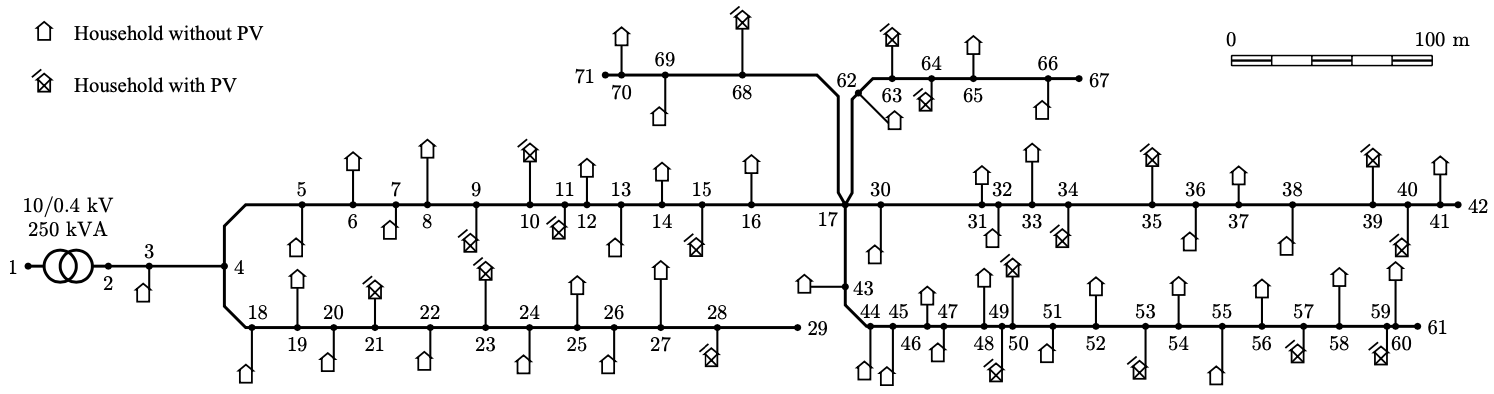
\includegraphics{Pictures/case70true.png}

\begin{itemize}
\tightlist
\item
  located in Belgium
\item
  bus 1 is omitted
\item
  62 households -\textgreater{} 62 active channels
\end{itemize}

\hypertarget{problem-formulation}{%
\chapter{Problem Formulation}\label{problem-formulation}}

\begin{itemize}
\tightlist
\item
  information in a directed graph \href{directed}{-\textgreater{} 3.1}
\item
  integer programming formulation \protect\hyperlink{IP}{-\textgreater{} 3.3}
\item
  local search heuristic algorithm \protect\hyperlink{combinatorial}{-\textgreater{} 3.4}
\end{itemize}

\begin{center}\rule{0.5\linewidth}{0.5pt}\end{center}

\begin{itemize}
\tightlist
\item
  remove overlapping edge \protect\hyperlink{overlapping}{-\textgreater{} 3.2}
\end{itemize}

\hypertarget{directed}{%
\section{Directed Graph}\label{directed}}

\textbf{weighted complete (directed) graph for a set of buses}

\begin{itemize}
\tightlist
\item
  any pair of buses -\textgreater{} edge -\textgreater{} \textbf{potential edges} to be selected
\item
  select a set of edges -\textgreater{} SA -\textgreater{} candidate
\item
  \textbf{impossible potential edge}
\item
  2-D Euclidean distance -\textgreater{} cable length -\textgreater{} weight
\end{itemize}

\textbf{feasible region}

\begin{itemize}
\tightlist
\item
  All the candidates (SAs).
\item
  Number of SAs is finite, making it a \protect\hyperlink{combinatorial}{combinatorial
  optimisation problem}.
\item
  Count number of SAs.
\end{itemize}

\hypertarget{overlapping}{%
\section{Remove Overlapping Edge}\label{overlapping}}

For example, in case-70:

\[
\begin{array}{lllll}
  \hline
  \textbf{shortest path} & <
  & \textbf{direct edge} & \times \textbf{threshold}
  & \text{-> } \textbf{remove direct edge} \\
  \hline
  \text{"b17‐b43-b29"} & < & \text{"b17-b29"} & \times 1.1
  & \text{-> remove "b17-b29"} \\
  \text{"b44‐b43-b29"} & > & \text{"b44-b29"} & \times 1.1
  & \text{-> keep "b44-b29"} \\
  \hline
\end{array}
\]

\begin{center}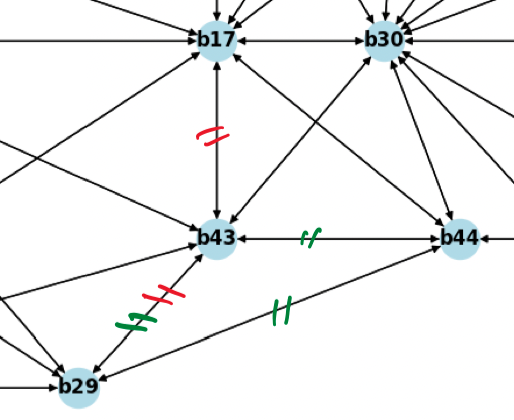
\includegraphics[width=0.6\linewidth]{Pictures/overlapGeth} \end{center}

However:

\begin{itemize}
\tightlist
\item
  446 possible potential edges
\item
  over \(10^{45}\) SAs
\end{itemize}

\begin{center}\rule{0.5\linewidth}{0.5pt}\end{center}

\protect\hyperlink{summary}{-\textgreater{} summary}

\hypertarget{IP}{%
\section{Integer Programming}\label{IP}}

Sets:

\[
\begin{array}{ll}
  \hline
  \textbf{symbol} & \textbf{definition} \\
  \hline
  \mathcal{E}
  & \text{all the potential edges} \\
  \mathcal{C}
  & \text{available snapshots} \\
  \mathcal{E}_\text{impossible}
  & \text{impossible potential edges} \\
  \hline
\end{array}
\]

Variables:

\[
\begin{array}{llll}
  \hline
  \textbf{symbol} & \textbf{definition} & \textbf{type} & \textbf{set} \\
  \hline
  x_{i j} & \text{whether to choose edge from i to j}
  & \text{binary} & \mathcal{E} \\
  \hline
\end{array}
\]

Constants:

\[
\begin{array}{lll}
  \hline
  \textbf{symbol} & \textbf{definition} & \textbf{set} \\
  \hline
  d_{i, j} & \text{Euclidean distance}
  & \mathcal{E} \\
  \hline
\end{array}
\]

\begin{center}\rule{0.5\linewidth}{0.5pt}\end{center}

\[
\begin{aligned}
  \min_{x_{i j} \forall (i, j) \in \mathcal{E}} \quad
    & (1 - \alpha) \sum_{(i, j) \in \mathcal{E}} d_{i j} x_{i j}
    + \alpha \mathcal{H}
    \left(\{x_{i j} \forall (i, j) \in \mathcal{E} \}, \mathcal{C} \right) \\
  \text{s.t.} \quad & \sum_{(i, j) \in \delta^{-}(j)} x_{i j} = 1
    \quad \forall j \in V^{\prime}
    \quad \text{(a directed forest)} \\
  & \sum_{(i, j) \in \delta^{-}(S)} x_{i j} \geq 1
    \quad \forall S \subseteq V^{\prime},|S| \geq 2
    \quad \text{(a connected graph)} \\
  & x_{i j} = 0
    \quad \forall (i, j) \in \mathcal{E}_\text{impossible}
    \quad \text{(remove impossible potential edges)}
\end{aligned}
\]

Two terms in the objective function:

\[
\begin{array}{lll}
  \hline
  \textbf{term} & \textbf{definition} & \textbf{coefficient} \\
  \hline
  (1 - \alpha) \sum_{(i, j) \in \mathcal{E}} d_{i j} x_{i j}
  & \text{total cable length of candidate}
  & 1 - \alpha \\
  \alpha \mathcal{H}
  \left(\{x_{i j} \forall (i, j) \in \mathcal{E} \}, \mathcal{C} \right)
  & \text{assessment of candidate}
  & \alpha \\
  \hline
\end{array}
\]

Three sets of constraints:

\begin{itemize}
\tightlist
\item
  First two sets ensure SA. \citep{fischetti1997branch}
\item
  Last set removes impossible potential edges.
\end{itemize}

\hypertarget{combinatorial}{%
\section{Local Search}\label{combinatorial}}

At least two possible values for \(\alpha\):

\[
\begin{array}{llll}
  \hline
  \textbf{value} & \textbf{term lefted} & \textbf{to find}
  & \textbf{disadvantage} \\
  \hline
  1
  & \mathcal{H}
  \left(\{x_{i j} \forall (i, j) \in \mathcal{E} \}, \mathcal{C} \right)
  & \text{ground truth}
  & \text{NP-hard and non-linear} \\
  0
  & \sum_{(i, j) \in \mathcal{E}} d_{i j} x_{i j}
  & \text{topology with min total cable length}
  & \text{cannot find ground truth} \\
  \hline
\end{array}
\]

Such two situations can be visualised:

\begin{center}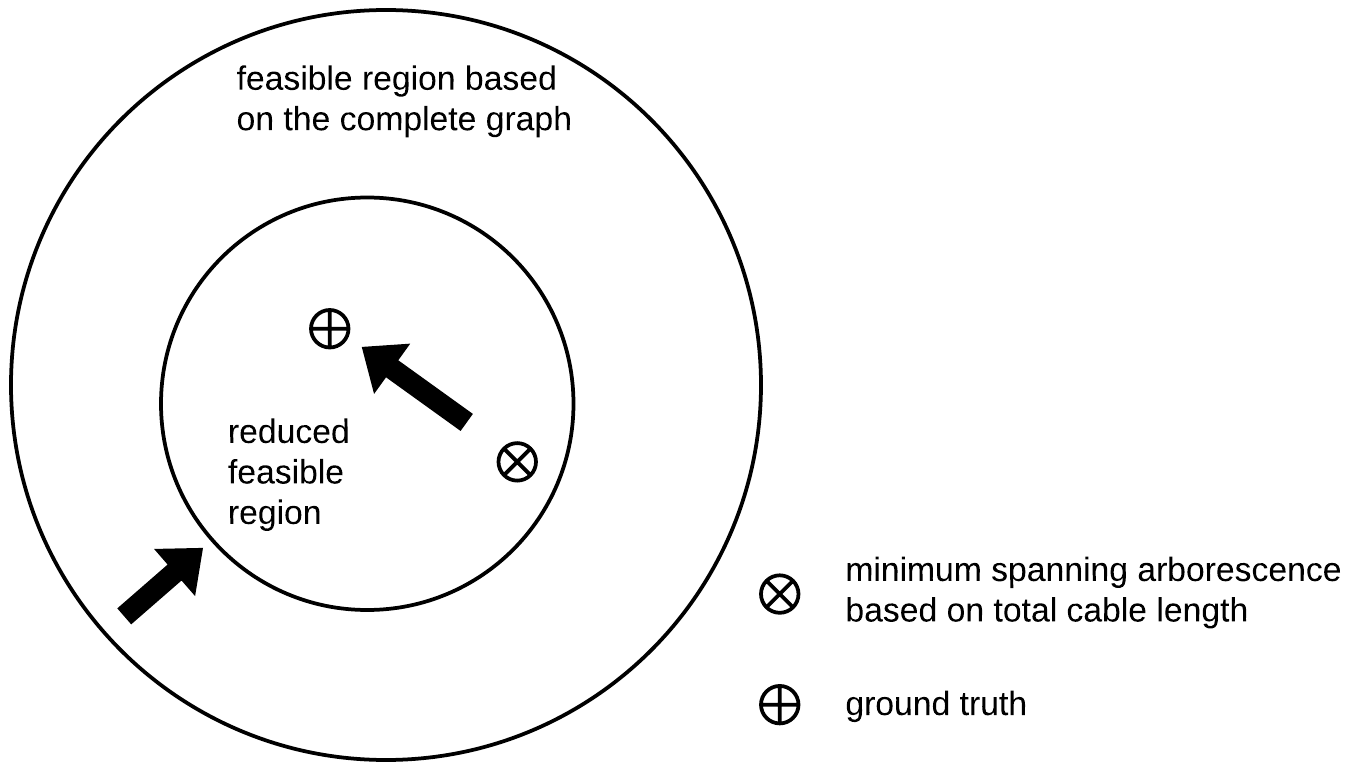
\includegraphics[width=0.7\linewidth]{Pictures/figFeasibleRegion} \end{center}

For this combinatorial optimisation problem, a \textbf{local search heuristic
algorithm} is proposed to move from \(\bigotimes\) to \(\bigoplus\).
\citep{michiels2007theoretical}

\begin{table}[H]
\centering
\begin{tabular}[t]{l|l|l}
\hline
function & what it does & in this project\\
\hline
objective & assess candidate & pseudo linearised power flow\\
\hline
neighbourhood & generate candidate & rank spanning arborescence\\
\hline
\end{tabular}
\end{table}

\begin{itemize}
\tightlist
\item
  Ground truth should be found before long.
\item
  Not in parallel.
\end{itemize}

\hypertarget{ac-power-flow}{%
\chapter{AC Power Flow}\label{ac-power-flow}}

\begin{itemize}
\tightlist
\item
  two essential matrices \protect\hyperlink{matrices}{-\textgreater{} 4.1}
\item
  bus impedance matrix \protect\hyperlink{BIM}{-\textgreater{} 4.2}
\item
  direct impedance method for power flow calculation \protect\hyperlink{power-flow}{-\textgreater{} 4.2}
\end{itemize}

\begin{center}\rule{0.5\linewidth}{0.5pt}\end{center}

Can be generalised for multi-phase model. \citep{hsieh2017matrix}

\hypertarget{matrices}{%
\section{Two Matrices}\label{matrices}}

current injection -\textgreater{} current flow:
\[
  \bar{\boldsymbol{I}}_{\text{edge}} =
  - \boldsymbol{K} \bar{\boldsymbol{I}}
\]

where \textbf{edge path incidence matrix (EPI)}, \(\boldsymbol{K}\).

voltage drop -\textgreater{} voltage:
\[
  \bar{\boldsymbol{V}} =
  \bar{\boldsymbol{V}}_{\text{zero}}
  - \boldsymbol{K}^{\top} \boldsymbol{\bar{Z}}_\text{edge}
  \bar{\boldsymbol{I}}_{\text{edge}} 
\]

where \textbf{edge impedance diagonal block matrix (EIDB)},
\(\boldsymbol{\bar{Z}}_\text{edge}\).

\begin{center}\rule{0.5\linewidth}{0.5pt}\end{center}

\begin{center}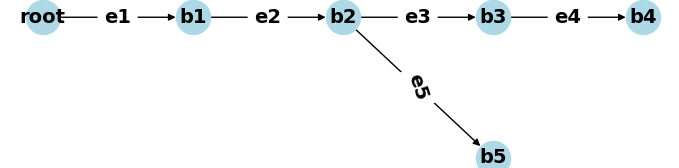
\includegraphics[width=0.7\linewidth]{Pictures/figCaseSixRaw} \end{center}

\[ \begin{aligned}
    \left[\begin{array}{l}
    \bar{I}_{\text{edge}, 1} \\
    \bar{I}_{\text{edge}, 2} \\
    \bar{I}_{\text{edge}, 3} \\
    \bar{I}_{\text{edge}, 4} \\
    \bar{I}_{\text{edge}, 5}
    \end{array}\right]
    = - \left[\begin{array}{lllll}
    1 & 1 & 1 & 1 & 1 \\
    0 & 1 & 1 & 1 & 1 \\
    0 & 0 & 1 & 1 & 0 \\
    0 & 0 & 0 & 1 & 0 \\
    0 & 0 & 0 & 0 & 1
    \end{array}\right]
    \left[\begin{array}{l}
    \bar{I}_{1} \\
    \bar{I}_{2} \\
    \bar{I}_{3} \\
    \bar{I}_{4} \\
    \bar{I}_{5}
    \end{array}\right]
\end{aligned} \]

\[ \begin{aligned}
  &
  \left[\begin{array}{c}
    \bar{V}_{1} \\
    \bar{V}_{2} \\
    \bar{V}_{3} \\
    \bar{V}_{4} \\
    \bar{V}_{5}
  \end{array}\right]
  -
  \left[\begin{array}{c}
    \bar{V}_\text{rate} \\
    \bar{V}_\text{rate} \\
    \bar{V}_\text{rate} \\
    \bar{V}_\text{rate} \\
    \bar{V}_\text{rate}
  \end{array}\right]
  =
  - \left[\begin{array}{ccccc}
    1 & 1 & 1 & 1 & 1 \\ 
    0 & 1 & 1 & 1 & 1 \\ 
    0 & 0 & 1 & 1 & 0 \\ 
    0 & 0 & 0 & 1 & 0 \\ 
    0 & 0 & 0 & 0 & 1
  \end{array} \right]^{\top}
  \left[\begin{array}{ccccc}
    Z_{\text{edge}, 1} & 0 & 0 & 0 & 0 \\
    0 & Z_{\text{edge}, 2} & 0 & 0 & 0 \\
    0 & 0 & Z_{\text{edge}, 3} & 0 & 0 \\
    0 & 0 & 0 & Z_{\text{edge}, 4} & 0 \\
    0 & 0 & 0 & 0 & Z_{\text{edge}, 5}
  \end{array}\right]
  \left[\begin{array}{l}
    \bar{I}_{\text{edge}, 1} \\
    \bar{I}_{\text{edge}, 2} \\
    \bar{I}_{\text{edge}, 3} \\
    \bar{I}_{\text{edge}, 4} \\
    \bar{I}_{\text{edge}, 5}
  \end{array} \right]
\end{aligned} \]

\begin{center}\rule{0.5\linewidth}{0.5pt}\end{center}

Alternating current power flow: \citep{conti2006voltage}
\[
  \bar{\boldsymbol{V}} = \bar{\boldsymbol{V}}_{\text{zero}}
    + \left( \boldsymbol{K}^{\top} \boldsymbol{\bar{Z}}_\text{edge}
    \boldsymbol{K} \right) \bar{\boldsymbol{I}}
\]

\hypertarget{BIM}{%
\section{Bus Impedance Matrix}\label{BIM}}

Alternating current power flow:
\[
  \bar{\boldsymbol{V}} = \bar{\boldsymbol{V}}_{\text{zero}}
    + \left( \boldsymbol{K}^{\top} \boldsymbol{\bar{Z}}_\text{edge}
    \boldsymbol{K} \right) \bar{\boldsymbol{I}}
\]

\begin{center}\rule{0.5\linewidth}{0.5pt}\end{center}

\textbf{Bus impedance matrix (BIM)}, \(\boldsymbol{\bar{Z}}\), is defined as:
\[ \begin{aligned}
  \boldsymbol{\bar{Z}}
    &= \boldsymbol{K}^{\top} \boldsymbol{\bar{Z}}_\text{edge}
    \boldsymbol{K} \\
    &= \boldsymbol{R} + j \boldsymbol{X}
\end{aligned} \]

where \textbf{bus resistance matrix (BRM)}, \(\boldsymbol{R}\): real part of entries
in BIM.

\hypertarget{power-flow}{%
\section{Direct Impedance Method}\label{power-flow}}

Five steps to build BIM:

\begin{enumerate}
\def\labelenumi{\arabic{enumi}.}
\tightlist
\item
  Define a unit impedance matrix.
\item
  Calculate edge impedance matrices for cables.
\item
  Build EIDB.
\item
  Obtain EPI based on topology.
\item
  Calculate BIM using EIDB and EPI.
\end{enumerate}

\hypertarget{fixed-point-method}{%
\subsection*{Fixed Point Method}\label{fixed-point-method}}
\addcontentsline{toc}{subsection}{Fixed Point Method}

The following procedure is repeated:
\[ \begin{aligned}
    \boldsymbol{\bar{I}} &= \boldsymbol{\underline{P}}
      \otimes \boldsymbol{\underline{V}}_\text{previous} \\
    \boldsymbol{\bar{V}}
    &= \boldsymbol{\bar{Z}} \boldsymbol{\bar{I}}
      + \boldsymbol{\bar{V}}_\text{zero} \\
    \epsilon
    &= \left( \boldsymbol{\bar{V}} - \boldsymbol{\bar{V}} \right)^\top
      \left( \boldsymbol{\bar{V}} - \boldsymbol{\bar{V}} \right)
\end{aligned} \]
until \(\epsilon\) is smaller than a pre-defined threshold.

\hypertarget{linearised-power-flow}{%
\chapter{Linearised Power Flow}\label{linearised-power-flow}}

\begin{itemize}
\tightlist
\item
  assessment of candidate \protect\hyperlink{assessment}{-\textgreater{} 5.3}
\end{itemize}

\begin{center}\rule{0.5\linewidth}{0.5pt}\end{center}

\begin{itemize}
\tightlist
\item
  bus resistance matrix \protect\hyperlink{BRM}{-\textgreater{} 5.1}
\item
  inversed bus resistance matrix \protect\hyperlink{brmInv}{-\textgreater{} 5.2}
\item
  error from linearisation \protect\hyperlink{error}{-\textgreater{} 5.4}
\end{itemize}

\hypertarget{BRM}{%
\section{Bus Resistance Matrix}\label{BRM}}

BRM of case-70:

\begin{itemize}
\tightlist
\item
  bus 2 -\textgreater{} root
\item
  69 PQ buses
\item
  207 channels -\textgreater{} 207 rows and 207 columns
\end{itemize}

\begin{center}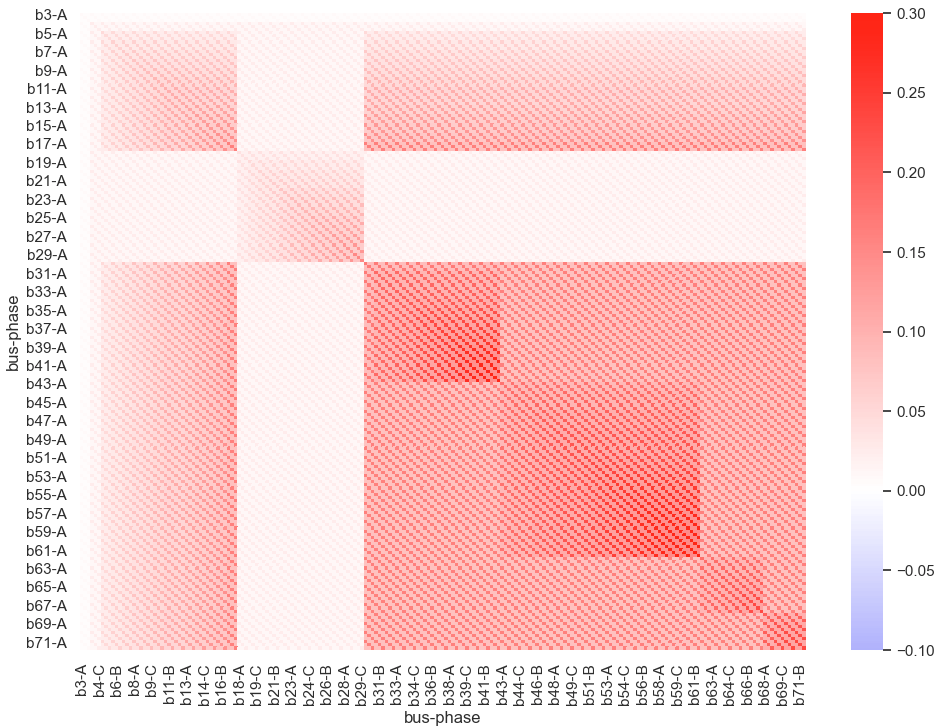
\includegraphics{Pictures/figHeatmapBRM} \end{center}

\hypertarget{LCA}{%
\subsection*{Lowest Common Ancestor Problem}\label{LCA}}
\addcontentsline{toc}{subsection}{Lowest Common Ancestor Problem}

Entry \((i, j)\) -\textgreater{} sum of edge resistances in the path from root to their lowest
common ancestor (LCA):
\[
R_{i, j}=\sum_{k \in U_{i} \cap U_{j}} R_{\text {edge }, k}
\]
where \(U_{i}\) is set of edges on the path from root to bus \(i\).

\begin{itemize}
\tightlist
\item
  Calcualted efficiently using LCA for all pairs.
\item
  Useful pattern.
\end{itemize}

For example,

\begin{center}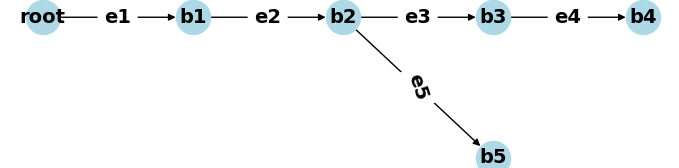
\includegraphics[width=0.7\linewidth]{Pictures/figCaseSix} \end{center}

\[ \begin{array}{ll}
  \hline
  \text{pair of buses} & \text{entry in BRM} \\
  \hline
  \text{b3-b5} & R_\text{e1} + R_\text{e2} \\
  \text{b4-b5} & R_\text{e1} + R_\text{e2} \\
  \hline
\end{array} \]

\begin{center}\rule{0.5\linewidth}{0.5pt}\end{center}

\protect\hyperlink{summary}{-\textgreater{} summary}

\hypertarget{brmInv}{%
\section{Pseudo Linearised Power Flow}\label{brmInv}}

Based on linearised power flow, \(\boldsymbol{V} = \boldsymbol{V}_\text{zero} + \frac{1}{V_\text{rate}} \boldsymbol{R} \boldsymbol{P}\):
\[ \begin{aligned}
    \boldsymbol{P}_\text{assess} =
    V_\text{rate} \boldsymbol{R}^{\top}
    \left( \boldsymbol{V} - \boldsymbol{V}_\text{zero} \right)
\end{aligned} \]
-\textgreater{} \textbf{pseudo linearised power flow}.

Inversed BRM for case-70:

\begin{center}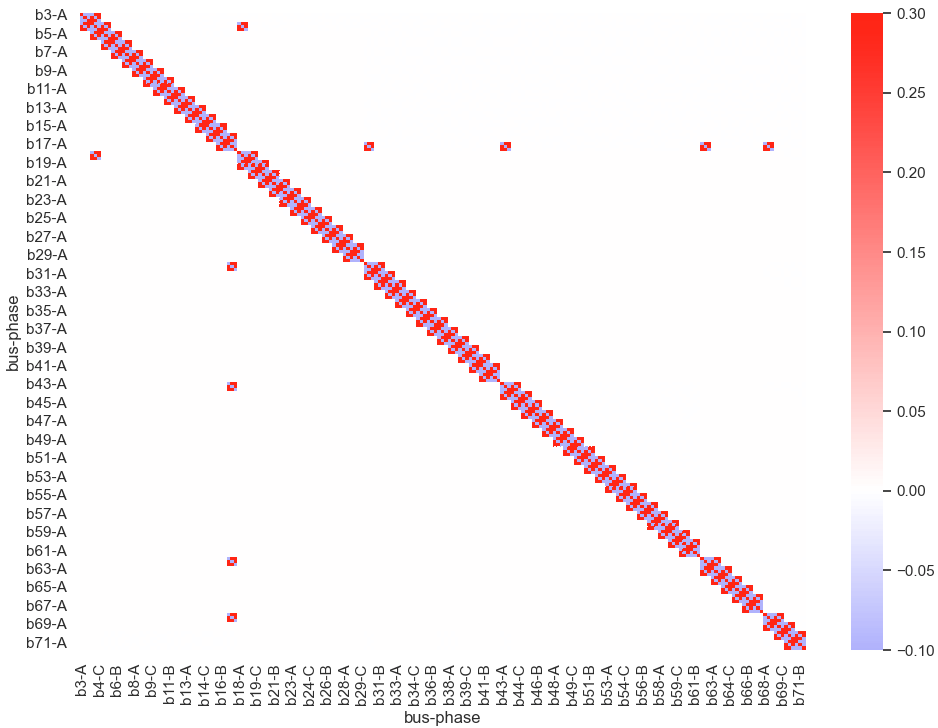
\includegraphics{Pictures/figHeatmapBrmInv} \end{center}

\begin{itemize}
\tightlist
\item
  Sparse.
\item
  Full rank.
\item
  Voltage magnitude at any channel can have a huge impact.
\item
  Useful pattern.
\end{itemize}

\begin{center}\rule{0.5\linewidth}{0.5pt}\end{center}

\protect\hyperlink{summary}{-\textgreater{} summary}

\hypertarget{assessment}{%
\section{Assessment of Candidate}\label{assessment}}

Linearised power flow:
\[ \begin{aligned}
  \boldsymbol{V} &= \boldsymbol{V}_\text{zero} + \frac{1}{V_\text{rate}}
    \left(
      \boldsymbol{K}^{\top} \boldsymbol{R}_\text{edge} \boldsymbol{K}
    \right) \boldsymbol{P} \\
  {} &= \boldsymbol{V}_\text{zero}
      + \frac{1}{V_\text{rate}} \boldsymbol{R} \boldsymbol{P}
\end{aligned} \]

\begin{center}\rule{0.5\linewidth}{0.5pt}\end{center}

\begin{itemize}
\tightlist
\item
  Calculate \(\boldsymbol{P}_\text{assess}\) using voltage magnitudes.
\item
  Compare with available power measurements.
\end{itemize}

\textbf{Mean squared error (MSE)}:
\[ \begin{aligned}
  \mathcal{H}(\boldsymbol{R}) =
  \left[
    (\boldsymbol{P}_\text{assess} - \boldsymbol{P}_\text{measure})
    \otimes \boldsymbol{O}
  \right]^\top
  \cdot \left[
    (\boldsymbol{P}_\text{assess} - \boldsymbol{P}_\text{measure})
    \otimes \boldsymbol{O}
  \right]
  / |\mathcal{O}|
\end{aligned} \]
where:

\begin{itemize}
\tightlist
\item
  \(\mathcal{O}\): set of observed active channels and inactive channels.
\item
  \(\boldsymbol{O}\): binary vector indicating observed active channels.
\end{itemize}

\begin{center}\rule{0.5\linewidth}{0.5pt}\end{center}

\protect\hyperlink{summary}{-\textgreater{} summary}

\hypertarget{error}{%
\section{Error from Linearisation}\label{error}}

Box plot:

\begin{itemize}
\tightlist
\item
  with respect to different number of observed active channels
\item
  based on ground truth and 50 snapshots\footnote{during 00:00:00 and 00:00:50 on Dec
    2, 2020 from Sonnen data set.}
\end{itemize}

\begin{center}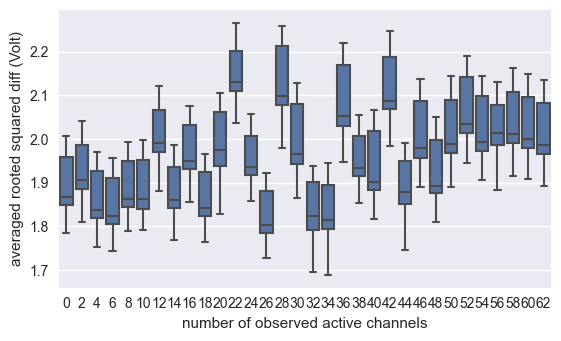
\includegraphics{Pictures/figErrorObsBRM} \end{center}

\begin{itemize}
\tightlist
\item
  \sout{Number of observed active channels.}
\item
  \(V_\text{rate}\) will increase the error dramatically.
\end{itemize}

\begin{center}\rule{0.5\linewidth}{0.5pt}\end{center}

\protect\hyperlink{summary}{-\textgreater{} summary}

\hypertarget{result-and-summary}{%
\chapter{Result and Summary}\label{result-and-summary}}

\begin{itemize}
\tightlist
\item
  result for case-70 \protect\hyperlink{result}{-\textgreater{} 6.1}
\item
  summary \protect\hyperlink{summary}{-\textgreater{} 6.2}
\end{itemize}

\hypertarget{result}{%
\section{Result for Case-70}\label{result}}

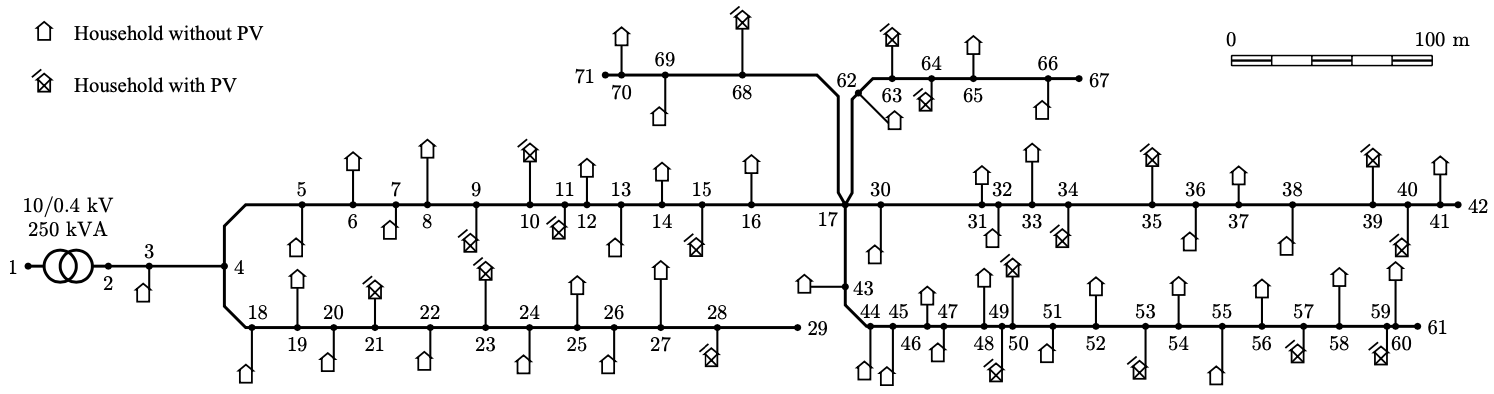
\includegraphics{Pictures/case70true.png}

\begin{itemize}
\tightlist
\item
  three new pairs, ``b29‐b44'', ``b68‐b14'', and ``b68‐b15''
\item
  144 potential edges in total
\item
  288 SAs rooted at bus 2
\item
  full observability
\end{itemize}

\begin{center}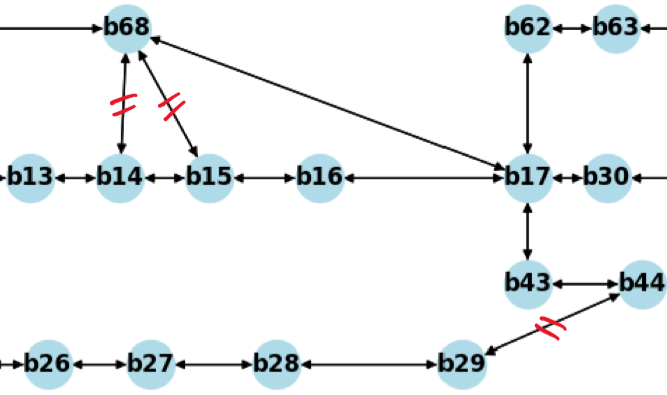
\includegraphics[width=0.55\linewidth]{Pictures/case70} \end{center}

Rank candidates according to total cable lengths:

\begin{center}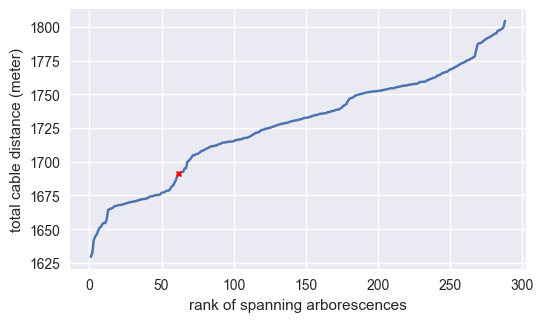
\includegraphics{Pictures/distances_288} \end{center}

Assessment based on 50 snapshots\footnote{during 00:00:00 and 00:00:50 on Dec 2, 2020
  from Sonnen data set.}:

\begin{center}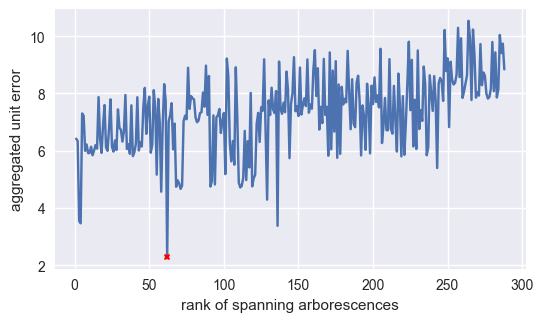
\includegraphics{Pictures/errors_288} \end{center}

\hypertarget{summary}{%
\section{Summary}\label{summary}}

\begin{itemize}
\tightlist
\item
  Topology inference -\textgreater{} combinatorial optimisation problem.
\item
  A new framework is proposed.
\item
  Core: local search heuristic algorithm.
\end{itemize}

Four steps:

\begin{enumerate}
\def\labelenumi{\arabic{enumi}.}
\tightlist
\item
  Shrink feasible region (reduce number of SAs).
\item
  Measure the size of feasible region.
\item
  Get candidates sequentially according to total cable lengths.
\item
  Assess candidates based on available measurements.
\end{enumerate}

Advantages:

\begin{itemize}
\tightlist
\item
  Robust to partial observability.
\item
  Integrate all kinds of information in weights and directions.
\end{itemize}

\hypertarget{issues}{%
\subsection*{Issues}\label{issues}}
\addcontentsline{toc}{subsection}{Issues}

\begin{enumerate}
\def\labelenumi{\arabic{enumi}.}
\tightlist
\item
  Too many candidates. (\protect\hyperlink{overlapping}{remove overlapping edges})
\item
  Full observability over voltage magnitudes. (\protect\hyperlink{BRM}{matrices with full
  rank})
\item
  Error in linearised power flow calculation. (\protect\hyperlink{error}{error from
  linearisation})
\end{enumerate}

\hypertarget{future-work}{%
\subsection*{Future Work}\label{future-work}}
\addcontentsline{toc}{subsection}{Future Work}

\begin{itemize}
\tightlist
\item
  How to detect more impossible potential edges. (for issue 1)
\item
  How to assess candidates based on a fraction. (for issue 2)
\item
  How to use voltage sensitivity matrix in linearised power flow. (for issue 3)
\end{itemize}

  \bibliography{bibliography.bib}

\end{document}
